%%%%%%%%%%%%%%%%%%%%%%%%%%%%%%%%%%%%%%%%%%%%%%%%%%%%%%%%%%%%
%%% ELIFE ARTICLE TEMPLATE
%%%%%%%%%%%%%%%%%%%%%%%%%%%%%%%%%%%%%%%%%%%%%%%%%%%%%%%%%%%%
%%% PREAMBLE 
\documentclass[9pt,lineno]{elife}
% Use the onehalfspacing option for 1.5 line spacing
% Use the doublespacing option for 2.0 line spacing
% Please note that these options may affect formatting.

\usepackage{lipsum} % Required to insert dummy text
\usepackage[version=4]{mhchem}
\usepackage{siunitx}
\DeclareSIUnit\Molar{M}
\usepackage{indentfirst} %I prefer to have indents following section headings, I find it to be more consistent in style throughout document

%%%%%%%%%%%%%%%%%%%%%%%%%%%%%%%%%%%%%%%%%%%%%%%%%%%%%%%%%%%%
%%% ARTICLE SETUP
%%%%%%%%%%%%%%%%%%%%%%%%%%%%%%%%%%%%%%%%%%%%%%%%%%%%%%%%%%%%
\title{Transcriptional dynamics of influenza virus infection in single cells}

\author[1]{Alistair B. Russell}
\author[2]{Cole Trapnell}
\author[1,2*]{Jesse D. Bloom}
\affil[1]{Basic Sciences Division and Computational Biology Program, Fred Hutchinson Cancer Research Center, Seattle, United States}
\affil[2]{Department of Genome Sciences, University of Washington, Seattle, United States}
\corr{jbloom@fredhutch.org}{}

% \presentadd[\authfn{5}]{eLife Sciences editorial Office, eLife Sciences, Cambridge, United Kingdom}

%%%%%%%%%%%%%%%%%%%%%%%%%%%%%%%%%%%%%%%%%%%%%%%%%%%%%%%%%%%%
%%% ARTICLE START
%%%%%%%%%%%%%%%%%%%%%%%%%%%%%%%%%%%%%%%%%%%%%%%%%%%%%%%%%%%%

\begin{document}

\maketitle

\begin{abstract}
Influenza virus infection induces large changes in cellular transcription.
Previously this has mostly been looked at using bulk measurements
Here we examine the process at the level of single cells.
We find extremely wide variation in the extent of viral gene transcription across infected cells.
IFN induction is very rare.
Some cellular pathways may be consistently altered in cells with high burden of viral transcripts.
Overall, highlights remarkable heterogeneity in the outcome of infection.
\end{abstract}


\section{Introduction}

Heterogeneity is important in a lot of cellular processes even when isogenic~\citep{shalek2013single,shalek2014single}.

Population (genetic) heterogeneity is also important. 
Viral quasispecies, cancer single-cell, etc.
Salmonella paper (PhoP).

Literature on viral burst-size heterogeneity.
This goes back to Delbruck, Andino polio paper~\citep{schulte2014single}, the MDCK / flu paper.

Discuss segmented nature of influenza.
Maybe in the context of how this could further increase heterogeneity because there is a lot of potential for entire genes to be missing.
Includes Yewdell and Lowen papers.

\section{Results}

\subsection{Strategy to measure mRNA in single virus-infected cells.}
We performed single-cell mRNA sequencing using a droplet-based system that physically isolates individual cells prior to reverse transcription.
Each droplet is associated with a unique \emph{cell barcode} that tags all mRNAs from that cell during reverse-transcription.
A random \emph{unique molecular identifier (UMI)} is additionally appended to each mRNA molecule during reverse transcription.
The 3' ends of the mRNAs are sequenced and mapped to the human and influenza transcriptomes to determine the transcript identities.
This information is combined with that provided by the UMIs and cell barcodes to quantify the number of molecules of each mRNA species that have been captured for each cell.

Infected cells will express viral as well as cellular mRNAs, however the cell barcodes and UMIs cannot distinguish whether a cell was initially infected by one or multiple viral particles.
We therefore engineered an influenza virus (strain A/WSN/1933) that additionally carried \emph{viral barcodes} consisting of synonymous mutations near the 3' end of each transcript (Figure~\ref{fig:workflow}A).
Critically, these synonymous mutations did not greatly impact viral growth kinetics (Figure~\ref{fig:workflow}B).
We infected A549 human lung carcinoma cells with an equal mix of the wildtype and synonymously barcoded viruses.
Cells infected by a single virion will exclusively express mRNAs from either wild-type or synonymously barcoded virus, whereas cells that are co-infected with multiple virions will often express mRNAs from both the wildtype and synonymously barcoded viruses (Figure~\ref{fig:workflow}C).
\begin{figure}
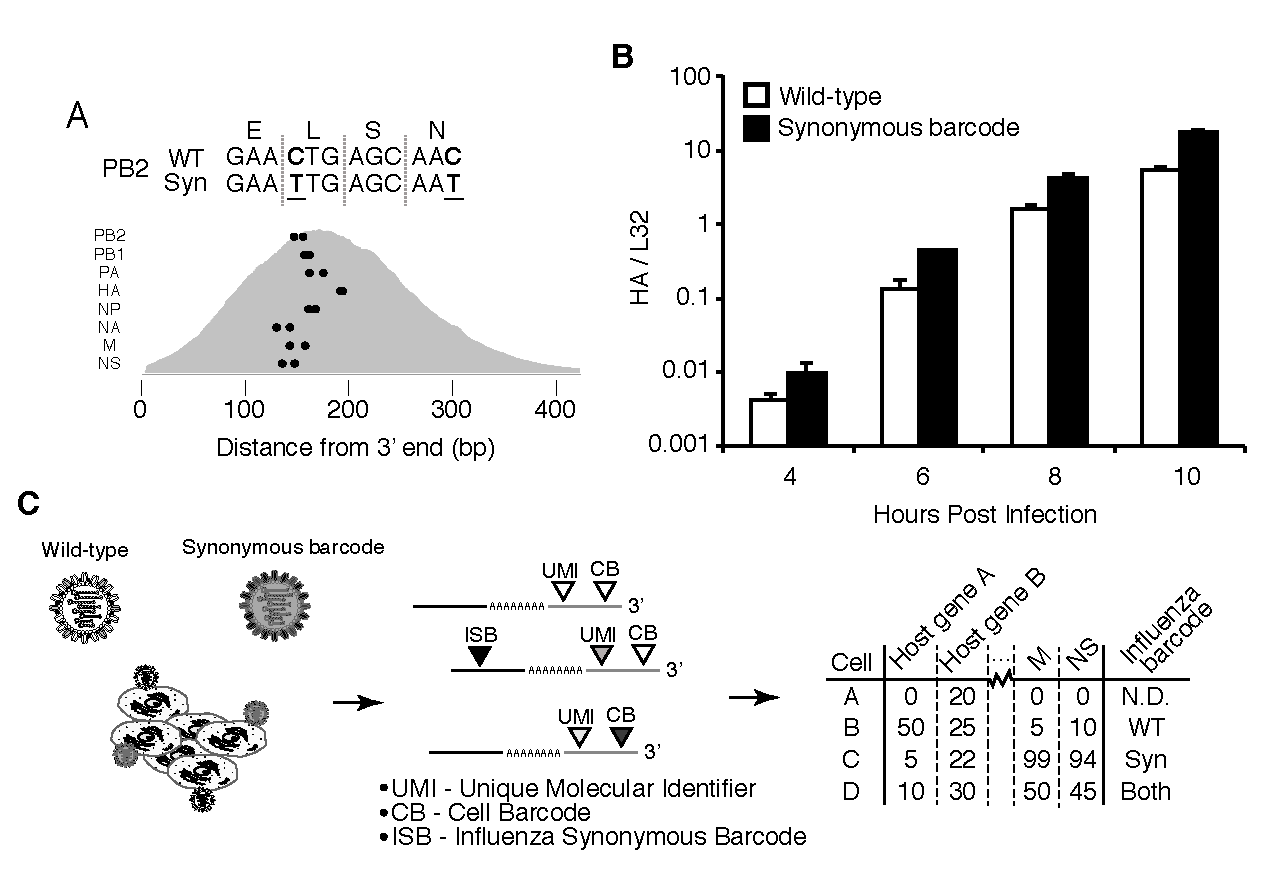
\includegraphics[width=0.8\linewidth]{figures/Workflow/workflow.pdf}
\caption{\label{fig:workflow} Experimental design.
{\bf (A)}  
We engineered a virus that carried two synonymous mutations near the 3' end of each mRNA.
At top are the specific mutations for the PB2 gene.
At bottom are locations of the synonymous mutations relative to the typical distribution of read depth for the 3'-end sequencing of the mRNA.
{\bf (B)} 
The wild-type and synonymously barcoded viruses transcribe their genes with similar kinetics. 
Shown is the abundance of the viral hemagglutinin (HA) transcript relative to the cellular housekeeping gene L32 as assessed by qPCR at the indicated time points in A549 cells infected at an MOI of 0.5 (as determined on MDCK-SIAT1 cells).
{\bf (C)}  
A549 cells were infected with an equal mixture of mutant and wild-type virus. 
Using reverse-phase emulsion, cells were physically separated and cDNA libraries were generated containing the indicated barcodes. 
The libraries were deep sequenced, and the data processed to create a matrix that gives the number of molecules of each transcript observed in each cell.
Infected cells were further annotated based on whether their viral mRNAs derived from the wildtype virus, the synonymously barcoded virus, or a mix of both.
Abbreviations: WT -- wild-type, Syn -- Synonymous Barcode.
}
\figdata{Sequences of wild-type and barcoded viruses are in \texttt{viralsequences.fasta}.}
\end{figure}

We also took care to generate stocks of virus that were relatively ``pure'' of defective particles.
Stocks of viruses typically contain an array of biologically active viral particles, some of which are defective for replication owing to mutations or deletions in essential viral genes.
These defective particles become prevalent when a virus is grown at high multiplicity of infection (MOI), where complementation permits the growth of otherwise deleterious genotypes.
To minimize the levels of defective particles, we propagated our viral stocks at low MOI for a relatively brief period of time~\citep{xue2016propagation}.
We then validated that our stocks exhibited greater purity of infectious particles than a stock propagated at high MOI by verifying that they had a higher ratio of infectious particles to both virion RNA (Figure~\ref{fig:viruspopulations}A) and particles capable of inducing expression of a single viral protein (Figure~\ref{fig:viruspopulations}B).
In addition, viral stocks with many defective particles are more immunostimulatory~\citep{tapia2013defective}.
We confirmed that our viral stocks induced much less interferon than a stock propagated at higher MOI (Figure~\ref{fig:viruspopulations}D).

\begin{figure}
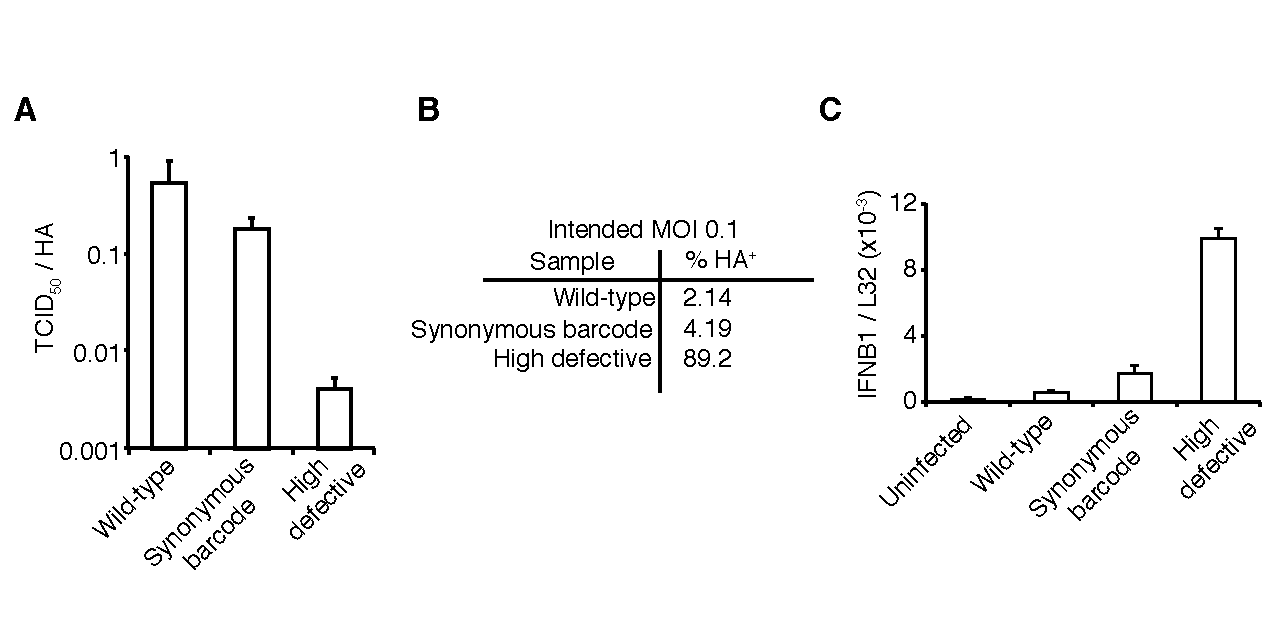
\includegraphics[width=0.7\linewidth]{figures/Validating_barcode_virus/validating_populations_D02.pdf}
\caption{\label{fig:viruspopulations} The viral stocks used in our experiments have relatively low numbers of defective particles. 
{\bf (A)}
Quantification of the relative amounts of physical viral particles and infectious particles.
Virions in the wildtype and synonymously barcoded viral stocks used in our experiments have a lower ratio of HA viral RNA to infectious particles compared to a high-defective stock propagated at high MOI.
Infectious particles were quantified by TCID50 on MDCK-SIAT1 cells, and HA vRNA by qPCR on virions. 
{\bf (B)} 
Quantification of the relative amounts of particles capable of expressing the viral protein HA to infectious particles.
A549 cells were infected with all three viral stocks at an MOI of 0.1 as calculated on MDCK-SIAT1 cells, and the percentage of cells expressing HA protein at 9 hours post-infection was quantified by antibody staining and flow cytometry.
{\bf (C)} 
Our viral stocks are less immunostimulatory than virus propagated at high MOI. 
Measurements of \textit{IFNB1} transcript by qPCR normalized to the housekeeping gene L32 in A549 cells at 10 hours post infection at an MOI of 0.5 as calculated on MDCK-SIAT1 cells.}
\figsupp[Flow cytometry data for calculating the percentage of HA-expressing cells.]{Longer caption}{\emph{HA-expression flow cytometry supplemental figure needs to be created.}}
\end{figure}

\subsection{Single infected cells show a wide range of expression of viral transcripts.}
We infected cells at a low multiplicity of infection with a mixture of the wildtype and synonymously barcoded viral populations and collected cells for mRNA sequencing at 6, 8, and 10 hours, including a replicate of the 8-hour timepoint.
We recovered roughly 3,000 to 4,000 cells for each sample (Figure~\ref{fig:cells}A). 
As expected, most cells expressed little or no viral mRNA (Figure~\ref{fig:cells}B).
However, a small fraction of cells expressed substantial numbers of viral mRNA molecules -- exceeding 10,000 in a few cells from the 10-hour timepoint (Figure~\ref{fig:cells}C). 
Consistent with known influenza replication kinetics, viral transcripts are observed to make up an increasing proportion of the total mRNA, although there was also very wide cell-to-cell variability in the number of viral transcripts at each time point (Figure~\ref{fig:cells}C).

\begin{figure}
\includegraphics[width=\linewidth]{figures/p_cell_mRNA_summary.pdf}
\caption{\label{fig:cells}
Overview of amounts of cellular and influenza virus mRNAs detected in each cell.
{\bf (A)} 
Number of cells captured for each sample.
{\bf (B)} 
Cumulative fraction plot showing the amount of mRNA derived from influenza for each sample.
In all samples, most cells had little or no influenza mRNA.
{\bf (C)} 
The number of cellular and viral mRNAs for each cell is plotted as a point.
The blue lines show the overall distribution of the number of cellular mRNAs per sample.
Cells that fell outside the red lines were removed as outliers.
At later timepoints, a small number of cells had a very high number of viral mRNAs.
}
\end{figure}

When calling infected cells we must be aware that uninfected cells could have small amounts of viral mRNA due to leakage of transcripts from lysed cells.
It is therefore important to establish a threshold for identifying truly infected cells.
We can do this by taking advantage of our use of both wild-type and synonymously barcoded viruses.
Reads derived from lysed cells will likely be drawn from both viral populations, and therefore cells that contain viral mRNA exclusibely acquired  through leakage should more frequently exhibit cooccurrence of viral barcodes.
Conversely, most infected cells will be infected by only a single virion, and so their reads should derive almost entirely from one of the two viral barcodes. 

Figure~\ref{fig:viralbarcodes}A shows the fraction of viral reads in individual cells that are derived from each viral barcode, and Figure~\ref{fig:viralbarcodes}B indicates the fraction of viral reads from the most abundant barcode in that cell.
As is clear from this figure, most cells expressing a large number of viral transcripts have these transcripts exclusively derived from just one of the viral barcodes -- indicating non-random partitioning as expected from viral infection.
A very small fraction of these cells express viral transcripts with both barcodes, presumably indicating rare co-infection events.
However, cells expressing a small number of viral transcripts often have a mixture of the two viral barcodes, as predicted by random partitioning from simple mRNA leakage (Figure~\ref{fig:viralbarcodes}B).
We therefore determined a threshold for the minimum amount of viral RNA that was present in cells in which the barcode partitioning appeared to result from infection rather than leakage (Figure~\ref{fig:viralbarcodes}C), and used this threshold to annotate all cells that we were confident were truly infected with virus.
Strikingly, among the infected the cells at each time point, a bare few contribute the majority of influenza transcripts (Figure~\ref{fig:viralbarcodes}D).
Specifically, at the 6 and 8-hour timepoints 10\% or less of the infected cells are responsible for over half the viral transcripts, while at the 10-hour timepoint 15\% of the infected cells produce over half the viral transcripts (Figure~\ref{fig:viralbarcodes}-Figure~supplement~\ref{figsupp:cumulfracflu}).


\begin{figure}
\includegraphics[width=\linewidth]{figures/p_frac_flu_summary.pdf}
\caption{\label{fig:viralbarcodes}
Synonymous barcodes near the 3' end of the influenza virus mRNAs were used to identify co-infection and distinguish true infections from cells that contained spurious viral reads.
{\bf (A)}
All cells with at least two viral mRNAs for which the viral barcode could be called, arranged in order of increasing influenza transcript counts.
Bar heights denote the viral mRNAs on a log\textsubscript{10} scale, bar coloring is linearly proportional to the fraction of viral mRNAs derived from either wild-type or synonymously barcoded virus.
{\bf (B)}
Same as (A), but now each bar is colored according to the relative proportions of the more common (major) and less common (minor) barcoded virus variant within each cell.
At low levels of viral mRNA there is often a roughly equal mix of barcodes, suggesting that many of these cells have simply picked up extracellular mRNA.
At higher levels of viral mRNA, cells generally associate with only one barcode, suggesting a single viral particle initiating infection, save for a few cells that are truly co-infected.
{\bf (C)}
We determined a cutoff for calling ``true'' infections by fitting a curve to the mean barcode purity of all cells with greater than a given fraction of their mRNA derived from virus.
We called the cutoff at the point at which purity stops increasing with the fraction of viral mRNA.
{\bf (D)}
The number of cells identified as infected and co-infected for each sample.
For all samples, the vast majority of cells were not infected, so for subsequent analyses we subsampled to a number of uninfected cells to either 50 or the number of infected cells, whichever was greater.
{\bf (E)} 
The distribution of the fraction of mRNA derived from virus for each sample for both infected and co-infected cells.
For all samples, there is a very wide distribution of the amount of viral mRNA.
}
\figsupp[Number of viral barcodes called.\label{figsupp:barcodescalled}]{
The number of viral barcodes called for each sample and influenza gene segment. 
Viral transcripts are classified as \emph{syn} if they mapped to a synonymously barcoded influenza transcript, \emph{wt} if they mapped to a wild-type influenza transcript, \emph{invalid} if multiple reads for the same UMI differed on the status of the viral barcode, and as \emph{uncalled} if none of the reads for that UMI overlapped the region of the viral transcript containing the viral barcode.
}{\includegraphics[width=\linewidth]{figures/synbarcodes_umistats.jpg}}
\figsupp[Cumulative distribution.\label{figsupp:cumulfracflu}]{
Description
}{\includegraphics[width=\linewidth]{figures/p_cumul_flu.pdf}}
\end{figure}

\subsection{Many infected cells are non-productive, explaining partially the broad distribution of viral gene expression.}

It is thought that a major driver of variation in influenza productivity is the segmented nature of the influenza genome.
Several groups have described that the majority of infections fail to express at least one of the eight influenza segments. 
Our data reveal a similar trend is true for this strain of influenza (Figure~\ref{fig:fluburdenbyflugene}A). 
When we bin cells according to absence of a given segment we observe that, unsurprisingly, absence of the tripartite polymerase (PB1, PA, PB2) and nuceoprotein (NP) correlates strongly with decreased influenza burden (Figure~\ref{fig:fluburdenbyflugene}B). 
This was true even when accounting for temporal variation, as seen by analyzing a single time point (10h) alone, with the caveat that there were too few NP absences detected to achieve statistical significance (supplemental figure).
Importantly, the gene products of all four of these segments are essential to the transition from primary mRNA transcription to replication and secondary mRNA transcription. 
This effect cannot be solely attributed to sampling error, as the polymerase genes exhibit the lowest expression and thus would be expected to be stochastically lost due to undersurveillance at much higher influenza transcript levels than would other genes. 
Nevertheless, while segment absence can partially explain extreme components of influenza variability resulting from an inability to fully engage in secondary transcription, absence of the remaining segments does not appear to have any significant impact on influenza burden.
Importantly, even cells expressing all eight segments still exhibit a wide distribution of influenza transcripts within each time point. We must instead therefore posit alternative mechanisms such as variability in host cells to explain the remainder of this distribution.  

We further wished to define metrics for absence for a given segment in order to understand the probability that a given infection could potentially produce infectious progeny. 
However, we decided to omit these calculations for PB1, PA, PB2, and NP due to the confounding effect of decreased influenza transcript abundance. 
In support of this decision, when we use cyclohexamide treatment to limit cells to primary transcription alone, we find a 2-3 log reduction in mRNA levels of PB1 or HA relative to a 10h time point (supplemental figure). 
We therefore lack confidence that our approach has the power to detect all semi-infectious events that result from a lack of polymerase or nucleoprotein segments.
Examining the remaining segments in only those cells expressing active polymerase, we find their absence at late timepoints (8h, 10h) ranges between 5 and 17 percent of infections, with reasonable agreement between samples (Figure~\ref{fig:fluburdenbyflugene}C).
Absence of a given segment appears to be an independent event, as presence of all four segments in an infection is well predicted by simply multiplying individual segment probabilities. 
We find our results within the range previously described for other influenza strains and consistent with the hypothesis that the majority of influenza infections are non-productive.







\begin{figure}
\includegraphics[width=\linewidth]{figures/p_flu_burden_flu_gene_merge.pdf}
\caption{\label{fig:fluburdenbyflugene}
The viral infection burden in individual cells as a function of the amount of each viral gene detected.
{\bf (A)} 
Fraction of mRNAs in each cell derived from virus as a function of the \emph{normalized} expression of each viral gene in that cell.
This plot shows that all cells with very high viral burden express all of the RNP genes, but some cells with high viral burden lack each of the other four viral genes.
{\bf (B)}
Statistical tests confirming that absence of viral RNP genes is significantly associated with reduced viral burden, but that the absence of the non-RNP genes does not lead to a clear decrease in viral burden.
{\bf (C)}
Per time point measurements of segment presence or absence in influenza infected cells that express all four genes of the polymerase complex. 
}
\figsupp[Like panel (B) but for the 10-hr sample only.\label{figsupp:10hrfluburdenbyflugene}]{
The absence of viral RNP genes but \emph{not} non-RNP genes remains significantly associated with reduced viral burden when we examine only the 10-hr sample, which is the single timepoint with the most data points.
The difference for NP is no longer statistically significant due to low counts of infected cells lacking NP, but the qualitative trend remains.
}{\includegraphics[width=\linewidth]{figures/p_10hr_flu_burden_flu_gene_test}}
\end{figure}


	
\subsection{Influenza mRNA Ratios are Tightly Controlled}
	
	This and other reports have described the considerable heterogeneity produced as influenza infection progresses in tissue culture models. 
	However, in stark contrast to our analyses above, the ratios of influenza mRNAs within a given cell appears to behave in a highly stereotyped fashion, with values roughly consistent with prior population-level measurements of influenza mRNA abundance. 
	Staggeringly, this is true whether or not cells are expressing mRNAs from all eight segments, at all three time points,  and, in cells running the gamut of infectious burden.
	Therefore while either noise in influenza replication or host variability can dramatically impact the amount of Influneza mRNA produced as a whole, these processes seem to, ignoring complete absence of a segment, act equally across the influenza genome.
	This is consistent with more limited measurements showing positive correlations between several segments in vRNA measurements in single cells.
	It would therefore be inadvisable to search for the sources of the broad distribution in influenza replication in those steps that can impact segments independently of one-another, such as noise in the transition to cRNA or vRNA production, but rather only in those processes that could impact the kinetics of all segments equivalently, such as transport to the nucleus or availability of cellular resources. 


\subsection{co-infection Occurs Early and Is Likely Adaptive For Influenza}
	While relatively rare in our dataset, those cells positively identified as containing both wild-type and synonymously barcoded influenza provide important insight into the nature of co-infection. 
	It has been posited that co-infection can rescue nonproductive infections, potentially by providing missing genome equivalents.
	\emph{Brooke et al}, for example observed increased co-occurrence of a given gene-segment pair as MOI was increased. 
	When we examine our coinfected cells, we observe a much higher rate of expression of all eight segments (metric).
	Consistent with this model, we also observe that if we consider only one barcode or the other, that many of these infections would instead have been non-productive. 
	Another observation that can be immediately procured is that, on the whole, co-infections have roughly balanced amounts of wild-type and barcoded segments. 
	Others have noted that windows for coinfection are relatively narrow, and, these data directly suggest that this window is specifically narrow with respect to cRNA and vRNA production.
	If significant replication of viral genomes had already occurred, one would expect a much wider distribution of ratios than those observed. 
	To support these observations, we generated a virus in which the HA segment was replaced by GFP, allowing us to detect coinfection by both wild-type and mutant virus by flow cytometry. 
	When we examine strictly co-infected cells, we observe that, as in our single-cell analysis, both HA and GFP are highly correlated -- indicating a tight window of coinfection.
	Moreover, a portion of the population expressing only low HA -- likely corresponding to primary transcription alone -- is greatly reduced. 
	These data give credence to the sentiments of others that non-productive events are perhaps just productive events waiting to occur, and that the true dynamics underlying descriptions of MOI are far more complex than we frequently give them credence, relying on assumptions that may frequently not accurately reflect reality.




\begin{figure}
\includegraphics[width=\linewidth]{figures/p_coinfection.pdf}
\caption{\label{fig:coexpression}
Frequency of each viral gene segment in co-infected cells with at least 5\% of their mRNA derived from influenza.
The bars indicate the logarithm of the number of each viral mRNA detected, and the bars are colored in proportion to the fraction of those mRNAs that are derived from either wildtype or synonymous barcoded virus.
}
\figdata{The raw data plotted in this figure are in \texttt{p\_co-infection.csv}.}
\end{figure}

\subsection{Relative expression of different viral genes}
Figure~\ref{fig:fluexpr} shows some of this.
Cite \citet{hatada1989control} to show our relative expressions are consistent with that.
Maybe show a panel with just the 8-segment infections.

Maybe add a figure breaking this down among timepoints.

\begin{figure}
\includegraphics[width=\linewidth]{figures/p_flu_expr.pdf}
\caption{\label{fig:fluexpr}
Expression of individual influenza genes in highly infected cells (at least 5\% of total mRNA is viral).
{\bf (A)} 
The fraction of total mRNA from each influenza gene for each cell.
{\bf (B)}
Box plots showing the fraction of viral mRNA per cell that is derived from each influenza gene taken over all highly expressed cells.
The black line at the notch in each box is the median, and the top and bottom of the box indicate the first and third quartiles.
}
\figdata{The raw data are in \texttt{p\_flu\_expr.csv}.}
\end{figure}

\subsection{Host stuff}

\begin{figure}
\includegraphics[width=\linewidth]{figures/p_small_tsne_merge.pdf}
\caption{\label{fig:tsne}
tSNE plots.
The layout is the same in all panels, but each panel colors the cells according to a different property.
{\bf (A), (B)}
Cells colored by the fraction of their mRNA that is viral.
{\bf (C)}
Cells colored by experimental sample.
While it is clear that cells from later timepoints often have more viral RNA, there are cells from earlier timepoints with a high viral burden and cells from late timepoints with a low viral burden.
{\bf (D)}
Cells colored by the number of type I and III interferon transcripts detected.
Only one cell has high expression of these interferons.
{\bf (E)}
Cells colored by the expression of the interferon-stimulate gene ISG15.
{\bf (F)}
For cells with at least 1\% of their reads from influenza, are the cells expressing the viral NS protein?
The one interferon-positive cell is lacking NS, but many other cells also lack NS but do not express interferon.
}
\end{figure}


\begin{figure}
\includegraphics[width=0.8\linewidth]{figures/p_cellular_heatmap.pdf}
\caption{\label{fig:cellulargenes}
Cellular genes that are differentially expressed with respect to the amount of influenza mRNA in individual cells infected with full influenza virus containing all eight genes.
Shown are all genes differentially expressed with $Q < 0.1$.}
\figdata{The full results of the differential expression test is in \texttt{p\_sig\_cellular\_genes.csv}.}
\figdata{The results of a gene-set analysis are in \texttt{p\_sig\_cellular\_genes.csv}.}
\end{figure}

\section{Discussion}

\lipsum[9]

\section{Methods and Materials}

Guidelines can be included for standard research article sections, such as this one. 

\lipsum[3]

\section{Some \LaTeX{} Examples}
\label{sec:examples}

Use section and subsection commands to organize your document. 
\LaTeX{} handles all the formatting and numbering automatically. 
Use ref and label commands for cross-references.

\subsection{Figures and Tables}


If you use the following prefixes for your \verb|\label|:
%
\begin{description}
\item[Figures] \texttt{fig:}, e.g.~\verb|\label{fig:view}|
\item[Tables] \texttt{tab:}, e.g.~\verb|\label{tab:example}|
\item[Equations] \texttt{eq:}, e.g.~\verb|\label{eq:CLT}|
\item[Boxes] \texttt{box:}, e.g.~\verb|\label{box:simple}|
\end{description}
%
you can then use the convenience commands as in \verb|\FIG{cells}|, \ to generate cross-reference \FIG{view}. 

\subsection{Citations}

LaTeX formats citations and references automatically using the bibliography records in your .bib file, which you can edit via the project menu. 
Use the \verb|\cite| command for an inline citation, like \cite{trapnell2014pseudo}, and the \verb|\citep| command for a citation in parentheses \citep{trapnell2014pseudo}. 
The LaTeX template uses a slightly-modified Vancouver bibliography style. 
If your manuscript is accepted, the eLife production team will re-format the references into the final published form. 
\emph{It is not necessary to attempt to format the reference list yourself to mirror the final published form.}


\section{Acknowledgments}

Additional information can be given in the template, such as to not include funder information in the acknowledgments section.

\nocite{*} % This command displays all refs in the bib file
\bibliography{references}


\end{document}
ommand displays all refs in the bib file
\bibliography{references}


\end{document}
